\chapter{Numerical results}
In the previous chapter, we discuss the implementation detail
and how we implement and apply LBM to various settings.
In this chapter, we show the visualizations and numerical results
obtained from the series experiments.

\section{Shear wave decay}

\begin{figure}[tb]
  \begin{center}
    \subfloat[$t = 0$]{
      \includegraphics[width=0.23\textwidth]{../log/sinusoidal_density/fig/density000000.pdf}
    }
    \subfloat[$t = 200$]{
      \includegraphics[width=0.23\textwidth]{../log/sinusoidal_density/fig/density000200.pdf}
    }
    \subfloat[$t = 400$]{
      \includegraphics[width=0.23\textwidth]{../log/sinusoidal_density/fig/density000400.pdf}
    }
    \subfloat[$t = 600$]{
      \includegraphics[width=0.23\textwidth]{../log/sinusoidal_density/fig/density000600.pdf}
    }\\
    \subfloat[$t = 800$]{
      \includegraphics[width=0.23\textwidth]{../log/sinusoidal_density/fig/density000800.pdf}
    }
    \subfloat[$t = 1000$]{
      \includegraphics[width=0.23\textwidth]{../log/sinusoidal_density/fig/density001000.pdf}
    }
    \subfloat[$t = 1200$]{
      \includegraphics[width=0.23\textwidth]{../log/sinusoidal_density/fig/density001200.pdf}
    }
    \subfloat[$t = 1400$]{
      \includegraphics[width=0.23\textwidth]{../log/sinusoidal_density/fig/density001400.pdf}
    }\\
    \subfloat[$t = 1600$]{
      \includegraphics[width=0.23\textwidth]{../log/sinusoidal_density/fig/density001600.pdf}
    }
    \subfloat[$t = 1800$]{
      \includegraphics[width=0.23\textwidth]{../log/sinusoidal_density/fig/density001800.pdf}
    }
    \subfloat[$t = 2000$]{
      \includegraphics[width=0.23\textwidth]{../log/sinusoidal_density/fig/density002000.pdf}
    }
    \subfloat[$t = 2200$]{
      \includegraphics[width=0.23\textwidth]{../log/sinusoidal_density/fig/density002200.pdf}
    }\\
    \caption{The density evolution for the Sinusoidal density at
      the $Y = 25$ in the lattice grid size of $(50, 50)$.
      The coefficients $\epsilon$ and $\rho_0$ are 
      set to $0.08$ and $0.5$ respectively.
      The relaxation term $\omega$ are set to $1.0$.
      \label{fig:sinusoidal-density}}
  \end{center}
\end{figure}


\begin{figure}[tb]
  \begin{center}
    \subfloat[$t = 0$]{
      \includegraphics[width=0.23\textwidth]{../log/sinusoidal_velocity/fig/vel000000.pdf}
    }
    \subfloat[$t = 200$]{
      \includegraphics[width=0.23\textwidth]{../log/sinusoidal_velocity/fig/vel000200.pdf}
    }
    \subfloat[$t = 400$]{
      \includegraphics[width=0.23\textwidth]{../log/sinusoidal_velocity/fig/vel000400.pdf}
    }
    \subfloat[$t = 600$]{
      \includegraphics[width=0.23\textwidth]{../log/sinusoidal_velocity/fig/vel000600.pdf}
    }\\
    \subfloat[$t = 800$]{
      \includegraphics[width=0.23\textwidth]{../log/sinusoidal_velocity/fig/vel000800.pdf}
    }
    \subfloat[$t = 1000$]{
      \includegraphics[width=0.23\textwidth]{../log/sinusoidal_velocity/fig/vel001000.pdf}
    }
    \subfloat[$t = 1200$]{
      \includegraphics[width=0.23\textwidth]{../log/sinusoidal_velocity/fig/vel001200.pdf}
    }
    \subfloat[$t = 1400$]{
      \includegraphics[width=0.23\textwidth]{../log/sinusoidal_velocity/fig/vel001400.pdf}
    }\\
    \subfloat[$t = 1600$]{
      \includegraphics[width=0.23\textwidth]{../log/sinusoidal_velocity/fig/vel001600.pdf}
    }
    \subfloat[$t = 1800$]{
      \includegraphics[width=0.23\textwidth]{../log/sinusoidal_velocity/fig/vel001800.pdf}
    }
    \subfloat[$t = 2000$]{
      \includegraphics[width=0.23\textwidth]{../log/sinusoidal_velocity/fig/vel002000.pdf}
    }
    \subfloat[$t = 2200$]{
      \includegraphics[width=0.23\textwidth]{../log/sinusoidal_velocity/fig/vel002200.pdf}
    }\\
    \caption{The velocity evolution for the Sinusoidal velocity at
      the $x = 25$ in the lattice grid size of $(50, 50)$.
      The coefficients $\epsilon$ and $\rho_0$ are 
      set to $0.08$ and $0.5$ respectively.
      The relaxation term $\omega$ are set to $1.0$.
      \label{fig:sinusoidal-velocity}}
  \end{center}
\end{figure}

\begin{figure}[tb]
  \begin{center}
    \subfloat[Sinusoidal density]{
      \includegraphics[width=0.48\textwidth]{../log/sinusoidal_density/fig/omega_vs_visc.pdf}
    }
    \subfloat[Sinusoidal velocity]{
      \includegraphics[width=0.48\textwidth]{../log/sinusoidal_velocity/fig/omega_vs_visc.pdf}
    }
    \caption{The simulated viscosity value 
    over various relaxation values $\omega$.\label{fig:omega-vs-visc}}
  \end{center}
\end{figure}

\begin{equation}
  \begin{aligned}
    \vv_x(y, t) & = \epsilon \exp
    \Biggl(
    -\nu
    \biggl(
      \frac{2\pi}{Y}
      \biggr)^2 t
    \Biggr) 
    \sin 
      \frac{2\pi y}{Y} \\
    \frac{\vv_x(y, t)}{
      \epsilon
      \sin  \frac{2\pi y}{Y}
    } & =  \exp
    \Biggl(
    -\nu
    \biggl(
      \frac{2\pi}{Y}
      \biggr)^2 t
    \Biggr) \\
    -\nu
    \biggl(
      \frac{2\pi}{Y}
      \biggr)^2 t
      &= 
    \log \frac{\vv_x(y, t)}{
      \epsilon
      \sin  \frac{2\pi y}{Y}
    } \\
    \nu
      &=
      - \frac{1}{t}
      \biggl(
        \frac{Y}{2\pi}
        \biggr)^2 
    \log \frac{\vv_x(y, t)}{
      \epsilon
      \sin  \frac{2\pi y}{Y}
    } \\
  \end{aligned}
\end{equation}

\section{Couette flow}

\begin{figure}[tb]
  \begin{center}
    \subfloat[$t = 0$]{
      \includegraphics[width=0.44\textwidth]{../log/couette_flow/fig/couette_flow000000.pdf}
    }
    \subfloat[$t = 200$]{
      \includegraphics[width=0.44\textwidth]{../log/couette_flow/fig/couette_flow000200.pdf}
    }\\
    \subfloat[$t = 400$]{
      \includegraphics[width=0.44\textwidth]{../log/couette_flow/fig/couette_flow000400.pdf}
    }
    \subfloat[$t = 600$]{
      \includegraphics[width=0.44\textwidth]{../log/couette_flow/fig/couette_flow000600.pdf}
    }\\
    \subfloat[$t = 800$]{
      \includegraphics[width=0.44\textwidth]{../log/couette_flow/fig/couette_flow000800.pdf}
    }
    \subfloat[$t = 1000$]{
      \includegraphics[width=0.44\textwidth]{../log/couette_flow/fig/couette_flow001000.pdf}
    }\\
    \subfloat[$t = 1200$]{
      \includegraphics[width=0.44\textwidth]{../log/couette_flow/fig/couette_flow001200.pdf}
    }
    \subfloat[$t = 1400$]{
      \includegraphics[width=0.44\textwidth]{../log/couette_flow/fig/couette_flow001400.pdf}
    }
    \caption{The velocity evolution at
      the $x = 25$ in the lattice grid size of $(50, 50)$.
      The wall velocity and the relaxation term $\omega$ are set
      to $50$ and $0.3$ respectively.
      \label{fig:couette-velocity-evolution}}
  \end{center}
\end{figure}


\section{Poiseuille flow}

\begin{figure}[tb]
  \begin{center}
    \subfloat[$t = 0$]{
      \includegraphics[width=0.31\textwidth]{../log/poiseuille_flow/fig/poiseuille_flow000000.pdf}
    }
    \subfloat[$t = 500$]{
      \includegraphics[width=0.31\textwidth]{../log/poiseuille_flow/fig/poiseuille_flow000500.pdf}
    }
    \subfloat[$t = 1000$]{
      \includegraphics[width=0.31\textwidth]{../log/poiseuille_flow/fig/poiseuille_flow001000.pdf}
    }\\
    \subfloat[$t = 1500$]{
      \includegraphics[width=0.31\textwidth]{../log/poiseuille_flow/fig/poiseuille_flow001500.pdf}
    }
    \subfloat[$t = 2000$]{
      \includegraphics[width=0.31\textwidth]{../log/poiseuille_flow/fig/poiseuille_flow002000.pdf}
    }
    \subfloat[$t = 2500$]{
      \includegraphics[width=0.31\textwidth]{../log/poiseuille_flow/fig/poiseuille_flow002500.pdf}
    }\\
    \subfloat[$t = 3000$]{
      \includegraphics[width=0.31\textwidth]{../log/poiseuille_flow/fig/poiseuille_flow003000.pdf}
    }
    \subfloat[$t = 3500$]{
      \includegraphics[width=0.31\textwidth]{../log/poiseuille_flow/fig/poiseuille_flow003500.pdf}
    }
    \subfloat[$t = 4000$]{
      \includegraphics[width=0.31\textwidth]{../log/poiseuille_flow/fig/poiseuille_flow004000.pdf}
    }
    \caption{The velocity evolution at
      the $x = 25$ in the lattice grid size of $(50, 50)$.
      The relaxation term $\omega$ are is
      to $0.7$.
      The density factor at the inlet and the density factor
      at the outlet are set to $0.3$ and $0.301$ respectively.
      \label{fig:poiseuille-velocity-evolution}}
  \end{center}
\end{figure}

\section{Flow in box with Sliding lid}
\subsection{}

\begin{figure}[tb]
  \begin{center}
    \subfloat[$t = 5000$]{
      \includegraphics[width=0.23\textwidth]{../log/sliding_lid_W0.10_visc0.03_size300/fig/vel_flow005000.pdf}
    }
    \subfloat[$t = 10000$]{
      \includegraphics[width=0.23\textwidth]{../log/sliding_lid_W0.10_visc0.03_size300/fig/vel_flow010000.pdf}
    }
    \subfloat[$t = 50000$]{
      \includegraphics[width=0.23\textwidth]{../log/sliding_lid_W0.10_visc0.03_size300/fig/vel_flow050000.pdf}
    }
    \subfloat[$t = 100000$]{
      \includegraphics[width=0.23\textwidth]{../log/sliding_lid_W0.10_visc0.03_size300/fig/vel_flow099500.pdf}
    }\\
    \subfloat[$t = 5000$]{
      \includegraphics[width=0.23\textwidth]{../log/sliding_lid_W0.20_visc0.06_size300/fig/vel_flow005000.pdf}
    }
    \subfloat[$t = 10000$]{
      \includegraphics[width=0.23\textwidth]{../log/sliding_lid_W0.20_visc0.06_size300/fig/vel_flow010000.pdf}
    }
    \subfloat[$t = 50000$]{
      \includegraphics[width=0.23\textwidth]{../log/sliding_lid_W0.20_visc0.06_size300/fig/vel_flow050000.pdf}
    }
    \subfloat[$t = 100000$]{
      \includegraphics[width=0.23\textwidth]{../log/sliding_lid_W0.20_visc0.06_size300/fig/vel_flow099500.pdf}
    }\\
    \subfloat[$t = 5000$]{
      \includegraphics[width=0.23\textwidth]{../log/sliding_lid_W0.30_visc0.09_size300/fig/vel_flow005000.pdf}
    }
    \subfloat[$t = 10000$]{
      \includegraphics[width=0.23\textwidth]{../log/sliding_lid_W0.30_visc0.09_size300/fig/vel_flow010000.pdf}
    }
    \subfloat[$t = 50000$]{
      \includegraphics[width=0.23\textwidth]{../log/sliding_lid_W0.30_visc0.09_size300/fig/vel_flow050000.pdf}
    }
    \subfloat[$t = 100000$]{
      \includegraphics[width=0.23\textwidth]{../log/sliding_lid_W0.30_visc0.09_size300/fig/vel_flow099500.pdf}
    }\\
    \subfloat[$t = 5000$]{
      \includegraphics[width=0.23\textwidth]{../log/sliding_lid_W0.40_visc0.12_size300/fig/vel_flow005000.pdf}
    }
    \subfloat[$t = 10000$]{
      \includegraphics[width=0.23\textwidth]{../log/sliding_lid_W0.40_visc0.12_size300/fig/vel_flow010000.pdf}
    }
    \subfloat[$t = 50000$]{
      \includegraphics[width=0.23\textwidth]{../log/sliding_lid_W0.40_visc0.12_size300/fig/vel_flow050000.pdf}
    }
    \subfloat[$t = 100000$]{
      \includegraphics[width=0.23\textwidth]{../log/sliding_lid_W0.40_visc0.12_size300/fig/vel_flow099500.pdf}
    }\\
    \caption{The stream plots of sliding lid
    with the lattice grid size of $(300, 300)$.
    Figure~(a) -- (d) are the results of 
    the viscosity $\nu = 0.03$ and the wall velocity $0.1$.
    Figure~(e) -- (h) are the results of 
    the viscosity $\nu = 0.06$ and the wall velocity $0.2$.
    Figure~(i) -- (l) are the results of 
    the viscosity $\nu = 0.09$ and the wall velocity $0.3$.
    Figure~(m) -- (p) are the results of 
    the viscosity $\nu = 0.12$ and the wall velocity $0.4$.
    Note that each setting is chosens to satisfy
    the Reynolds number 1000.
      \label{fig:sliding-lid-velocity-evolution}}
  \end{center}
\end{figure}

\subsection{}
\begin{figure}
  \centering
  \includegraphics[width=0.68\textwidth]{../log/sliding_lid_W0.10_visc0.03_size300/fig/scaling_test.pdf}
  \caption{The scaling test of the sliding lid simulation. The grid size is $300 \times 300$.}
  \label{fig:sliding-lid-scaling}
\end{figure}

